\documentclass[12pt]{article}

\usepackage[utf8]{vietnam}
\usepackage{indentfirst}
\usepackage[hyphens]{url}
\usepackage{float}
\usepackage{graphicx}

\title{BÁO CÁO BTCN-02: THUẬT TOÁN TÔ MÀU}
\author{Nguyễn Trần Hậu - MSSV 1612180}
\date{12/12/2018}

\begin{document}

\maketitle

\section{Thuật toán Scan line}

\subsection{Đa giác}
Mỗi đỉnh trên đa giác có tọa độ ($x$, $y$).
$y\_min$ là giá trị y nhỏ nhất của tập tất cả các đỉnh của đa giác,
$y\_max$ tương tự là giá trị y lớn nhất.

Thuật toán Scan line yêu cầu dùng đường thẳng song song với Ox, quét qua đa giác,
bắt đầu từ đường thẳng $y = y\_min$ đến đường thẳng $y = y\_max$.

Mỗi lần quét qua, cần tính giao điểm của đường thẳng quét qua với các cạnh của đa giác.
Đưa giá trị $x$ của các giao điểm này vào một list, sau đó sắp xếp lại từ nhỏ đến lớn.
Lấy từng cặp trong list (như phần tử 0 và phần tử 1, phần tử 2 và phần tử 3, phần tử 4 và phần tử 5, ...)
kết hợp giá trị $y$ là đường thẳng quét qua để tạo thành các cặp điểm.
Sau đó tô màu tất cả các điểm nằm giữa 2 điểm thuộc một cặp.

Đối với trường hợp giao điểm tìm được là một đỉnh của đa giác.
Nếu đỉnh đó thấp/cao hơn hai đỉnh bên cạnh (đường thẳng quét qua cắt 2 cạnh tại đỉnh chung)
thì thêm giá trị $x$ của đỉnh đó vào list như giao điểm bình thường;
cuồi cùng trong list, giá trị $x$ của đỉnh đó lặp lại 2 lần.
Những đỉnh còn lại, chỉ thêm giá trị $x$ của đỉnh vào list nếu giá trị $x$ chưa xuất hiện trong list;
cuối cùng trong list, giá trị $x$ của đỉnh chỉ xuất hiện đúng 1 lần.

Mã giả thuật toán Scan line áp dụng cho đa giác: \\
\texttt{lặp y từ y\_min đến y\_max} \\
\texttt{\indent khởi tạo list rỗng} \\
\texttt{\indent lặp v là cạnh của đa giác} \\
\texttt{\indent\indent p là giao điểm của v và đường thẳng y} \\
\texttt{\indent\indent nếu p là đỉnh mà không cao/thấp hơn 2 đỉnh kề} \\
\texttt{\indent\indent\indent thêm p.X vào list nếu p.X chưa có trong list} \\
\texttt{\indent\indent còn lại thì thêm p.X vào list} \\ \\
\texttt{\indent sắp xếp lại list từ nhỏ đến lớn} \\ \\
\texttt{\indent lặp i từ 0 đến kích thước list - 2, mỗi lần lặp i tăng 2} \\
\texttt{\indent\indent tô màu tất cả điểm nằm giữa list[i] và list[i + 1]}

\subsection{Ellipse}
Ellipse khá dễ so với trường hợp đa giác.
Vì mỗi lần có đường thẳng song song với Ox quét qua, luôn có 2 giao điểm.
Trường hợp đường thẳng quét qua là tiếp tuyến với ellipse, thì vẫn tính giao điểm 2 lần.
Áp dụng tương tự như trường hợp đa giác, chỉ khác là không cần xét giao điểm có là đỉnh hay không
(vì ellipse không có đỉnh). Cuối cùng tô màu tất cả các điểm nằm giữa 2 giao điểm tạo bởi đường thẳng quét qua.

Mã giả thuật toán Scan line áp dụng cho ellipse: \\
\texttt{lặp y từ y\_min đến y\_max} \\
\texttt{\indent p1, p2 là giao điểm của ellipse và đường thẳng y} \\
\texttt{\indent tô màu tất cả điểm nằm giữa p1 và p2}

\section{Thuật toán Boundary fill}
Thuật toán Boundary fill giống như vết dầu loang.
Bắt đầu với một điểm hạt giống (seed) nằm trong hình,
sau đó xét 4 điểm xung quanh (trên, dưới, trái phải) điểm hạt giống,
rồi lại xét tiếp 4 điểm xung quanh ...

Mã giả thuật toán Boundary fill: \\
\texttt{BoundaryFill(điểm p, màu viền, màu cần tô)} \\
\texttt{\indent nếu màu của điểm p khác màu viền và khác màu cần tô} \\
\texttt{\indent\indent tô màu điểm p bằng màu cần tô} \\
\texttt{\indent\indent BoundaryFill(điểm trên p, màu viền, màu cần tô)} \\
\texttt{\indent\indent BoundaryFill(điểm dưới p, màu viền, màu cần tô)} \\
\texttt{\indent\indent BoundaryFill(điểm bên phải p, màu viền, màu cần tô)} \\
\texttt{\indent\indent BoundaryFill(điểm bên trái p, màu viền, màu cần tô)}

Đối với đa giác, tìm điểm hạt giống từ những điểm lân cận một đỉnh bất kì.
Đối với ellipse, điểm hạt giống có thể chọn là tâm của ellipse.

\section{Thuật toán Boundary fill khử đệ quy}
Để khử đệ quy cho thuật toán Boundary fill, cần sử dụng stack.

Đầu tiên push điểm hạt giống vào trong stack.
Mỗi lần lặp, pop từ stack ra một điểm.
Rồi xét điều kiện tô được hay không mà quyết định đưa vào stack 4 điểm xung quanh.

Mã giả thuật toán Boundary fill khử đệ quy: \\
\texttt{khởi tạo stack} \\
\texttt{push điểm hạt giống vào stack} \\
\texttt{lặp cho đến stack rỗng} \\
\texttt{\indent pop điểm p ra khỏi stack} \\
\texttt{\indent nếu điểm p khác màu viền và khác màu cần tô} \\
\texttt{\indent\indent tô màu điểm p bằng màu cần tô} \\
\texttt{\indent\indent push 4 điểm trên, dưới, trái, phải của p vào stack}

\section{So sánh}
So sánh 3 thuật toán bằng thời gian chạy của 3 thuật toán với các đa giác, ellipse được vẽ random.

\begin{figure}[H]
\centering
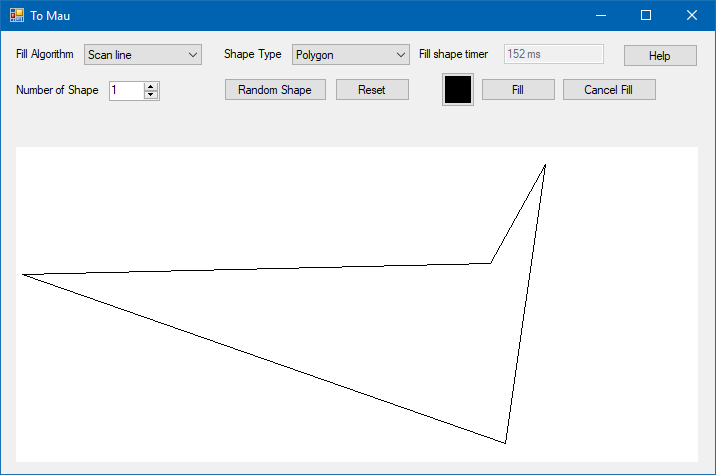
\includegraphics[width=\textwidth]{images/hinh1.png}
\caption{Đa giác 1}
\end{figure}

\begin{figure}[H]
\centering
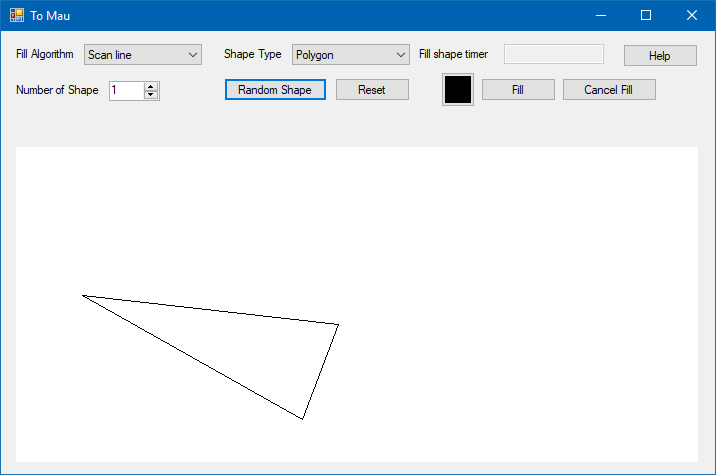
\includegraphics[width=\textwidth]{images/hinh2.png}
\caption{Đa giác 2}
\end{figure}

\begin{figure}[H]
\centering
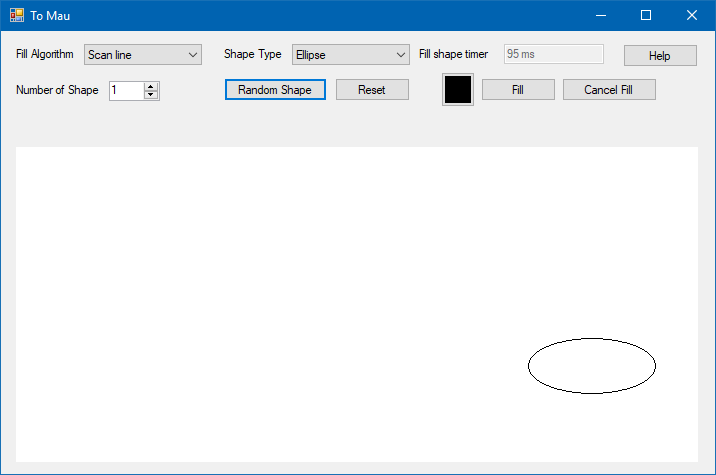
\includegraphics[width=\textwidth]{images/hinh3.png}
\caption{Ellipse 1}
\end{figure}

\begin{table}[H]
\begin{tabular}{| c || c | c | c |}
\hline
Hình & Scan line & Boundary fill & Boundary fill khử đệ quy \\
\hline \hline
Đa giác 1 & 26ms & (lỗi quá bộ nhớ) & 152ms \\
\hline
Đa giác 2 & 10ms & (lỗi quá bộ nhớ) & 38ms \\
\hline
Ellipse 1 & 3ms & (lỗi quá bộ nhớ) & 18ms \\
\hline
Ellipse 2 & 3ms & (lỗi quá bộ nhớ) & 22ms \\
\hline
\end{tabular}
\caption{Thời gian vẽ hình của từng thuật toán}
\end{table}

\textbf{Kết luận}: Toàn bộ lần tô màu thử, thuật toán Boundary fill đều bị lỗi quá bộ nhớ.
Nguyên nhân là do gọi đệ quy quá nhiều lần.
Thời gian chạy thuật toán Scan line ít hơn thời gian chạy thuật toán Boundary khử đệ quy.

\begin{thebibliography}{9}

\bibitem{b0} Slide Clipping and Filling Color

\bibitem{b1} Scan-Line \\
\url{https://www.techfak.uni-bielefeld.de/ags/wbski/lehre/digiSA/WS0607/3DVRCG/Vorlesung/13.RT3DCGVR-vertex-2-fragment.pdf}

\bibitem{b2} Flood Fill algorithm (using C\#.Net) \\
\url{https://simpledevcode.wordpress.com/2015/12/29/flood-fill-algorithm-using-c-net/}

\end{thebibliography}

\end{document}